\chapter{System Design}\label{chapter:general_design_decisions}

\section{Core Design Decisions}
The Framework is designed to be distributed in nature with the concepts of Actors. It should follow the standard actor programming concept and have the inherently distributed nature. The framework itself should be built using the concept of message passing to alleviate any possibility of concurrency issues, thus thread-safe.
\begin{itemize}
  \item The framework does not guarantee the delivery of a message.
  \item All the messages send by the framework is based on ‘fire and forget’concept.
  \item A message is delivered at most once.
  \item A message is always routed through Message Queuing System, even though the target isolate can belong to same isolate system in the same logical or physical node.
  \item A message is only fetched after an isolate sends a PULL request. Nonetheless, the delivery of message to an isolate is based on the implementation of the load balancer \textendash{} i.e. router.
\end{itemize}

\section{Architectural Overview}
\begin{figure}[H]
  \centering
  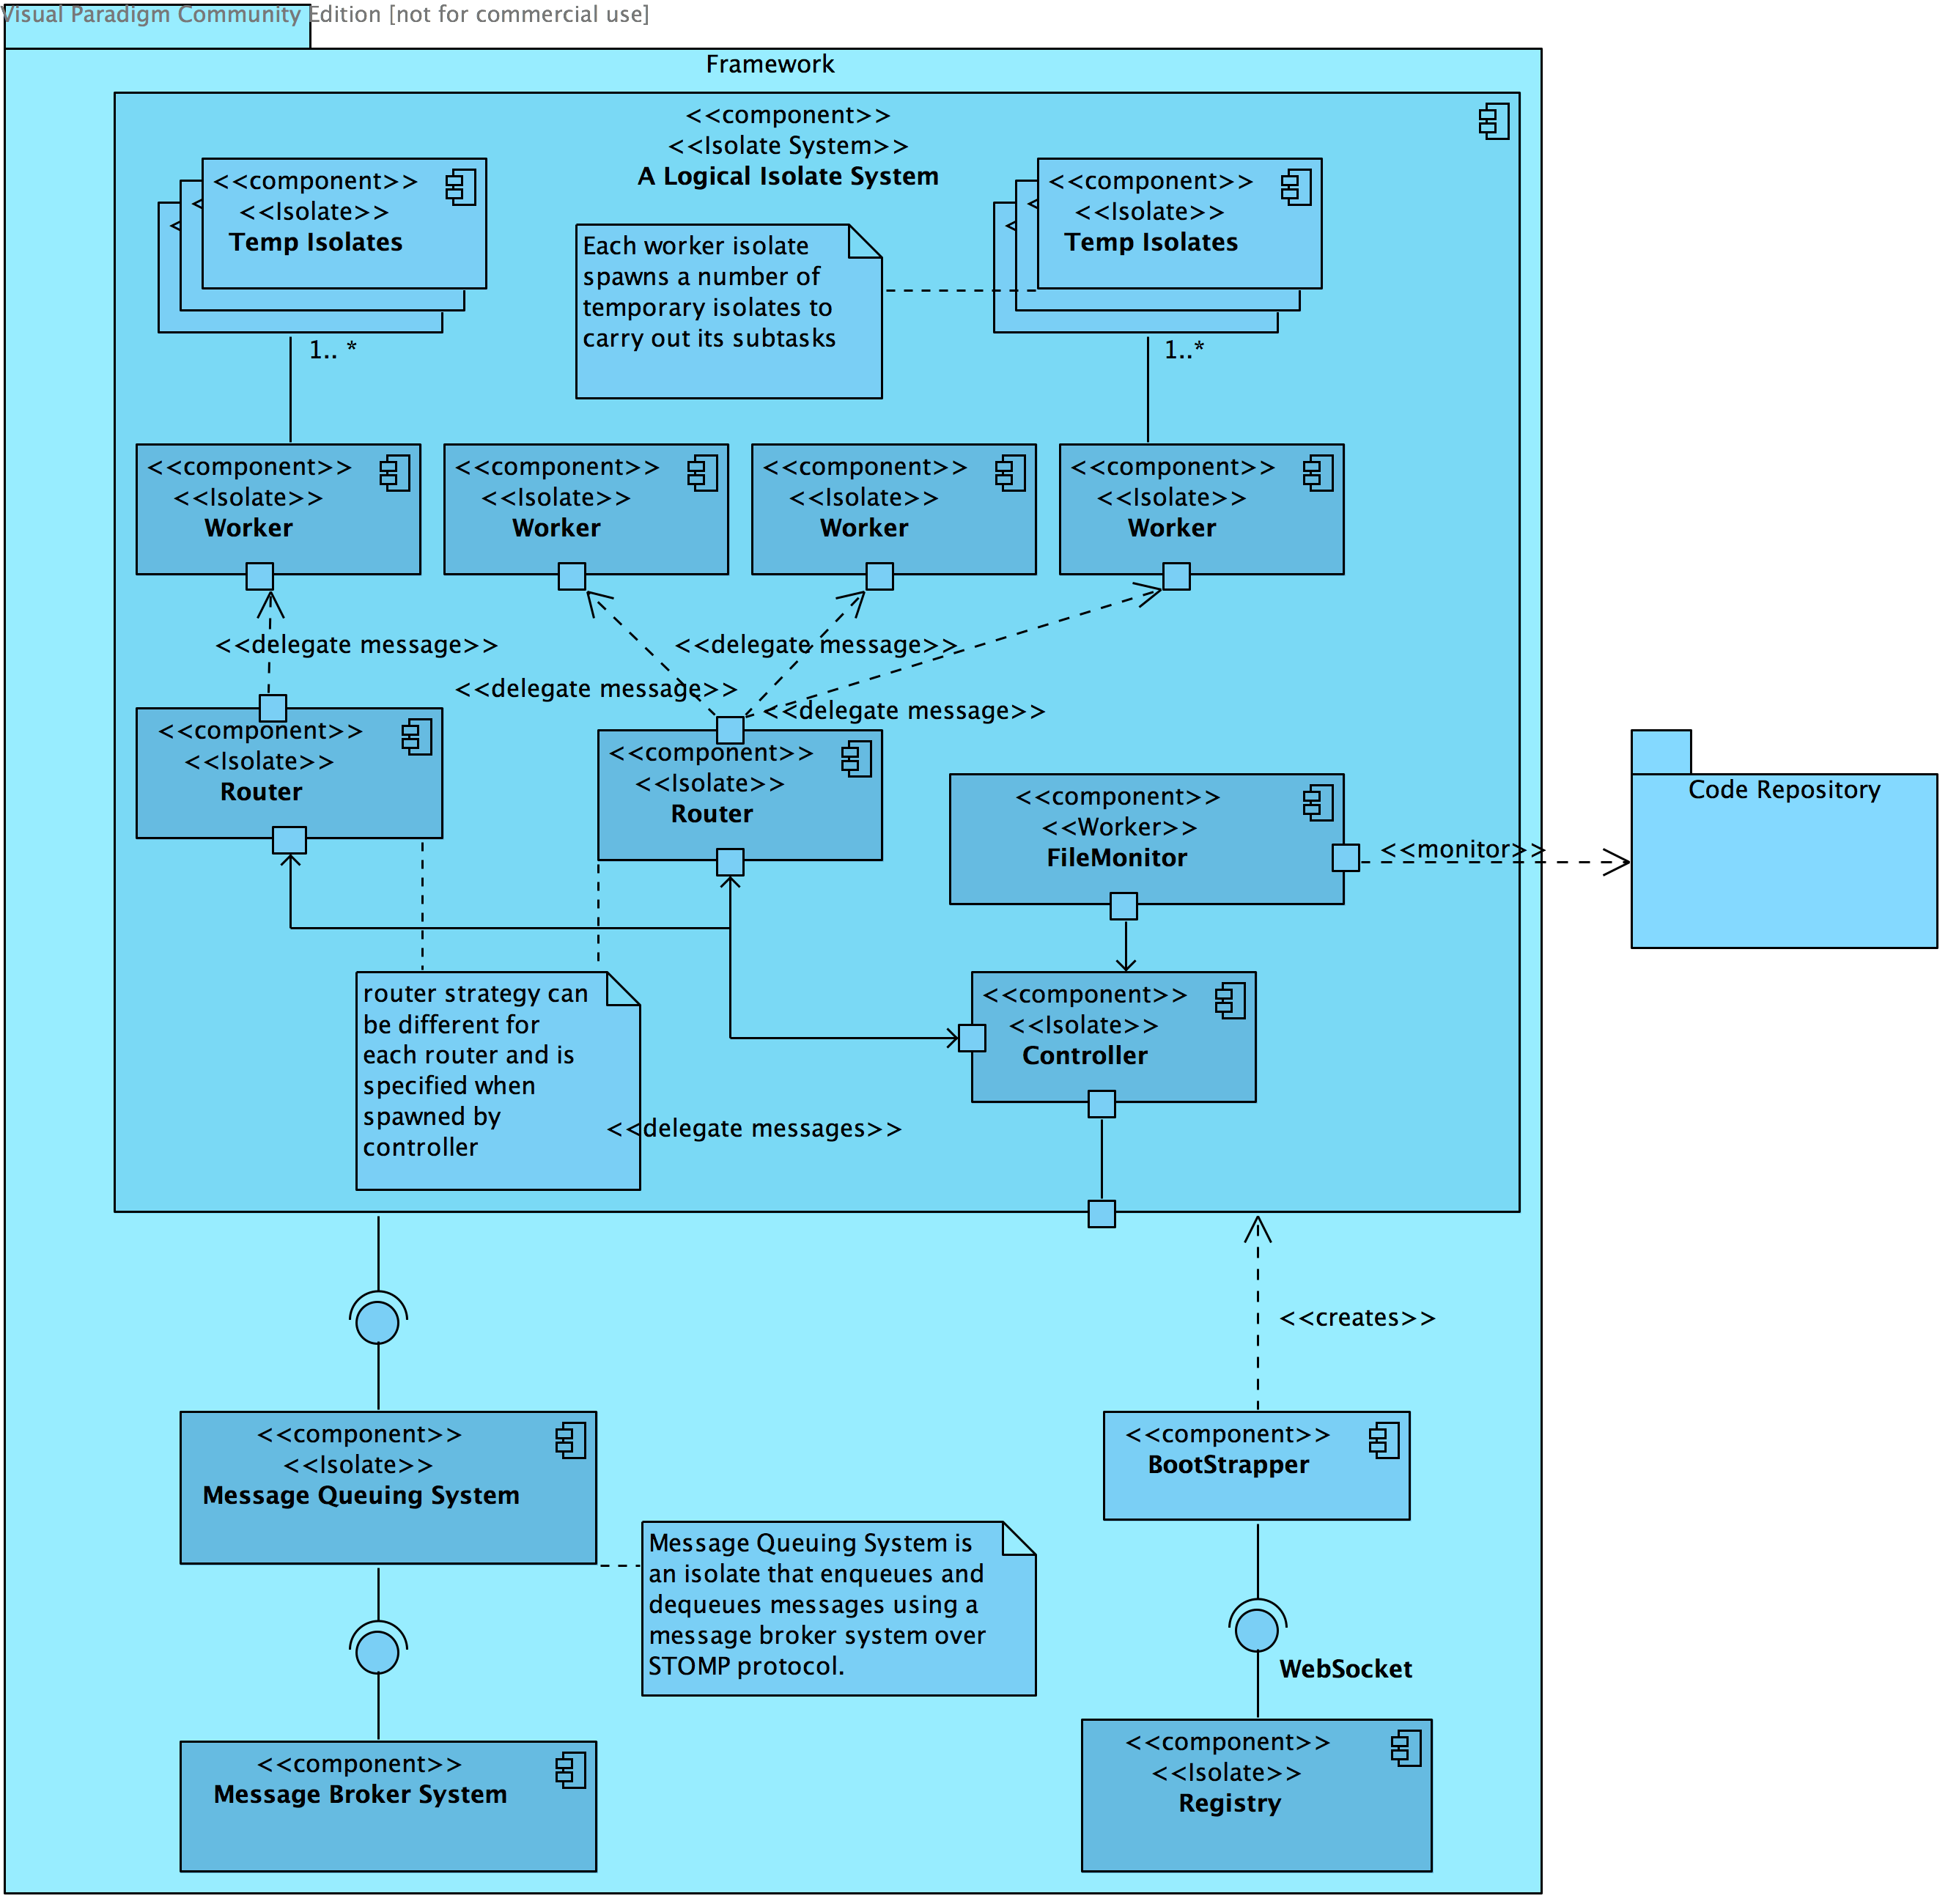
\includegraphics[width=1\textwidth]{figures/componentDiagram}
  \caption[architecture]{Architecture of the framework}
\end{figure}
\section{The Framework}
The framework comprises of an Isolate System, a Registry, a Message Queuing System and a Message Broker System.
  \subsection{IsolateSystem}
  An Isolate System is analogous to an actor system. Just as actor system is comprised of a group of actors working together, a group of related isolates form an isolate system. A ‘Bootstrapper’ in physical node can bootstrap several Isolate Systems. Nevertheless, a logical Isolate System is not limited to a single physical node. The isolates spawned by an Isolate System can be distributed across several remote systems.
  Each Isolate system has its unique id, which is a UUID. It is generated when the isolate system is bootstrapped. For bootstrapping, isolate system needs the WebSocket path to Message Queuing System, and a ‘name’ for itself. The name should not be confused with the uniqueId as IsolateSystem with same name can exist in other nodes but the uniqueId is unique for a particular instance of Isolate System.
  When an Isolate System is bootstrapped, it does several things. It generates a new Id which is unique for itself, then opens up a ‘ReceivePort’ and listens for any messages in that port so that it can receive to incoming messages from ‘Controller’. Then it tries to connect to Message Queuing System. If the Message Queuing System could not be connected, it simply keeps on retrying at certain interval. Furthermore, if after establishing connection with the MQS, the connection is lost in between because of a network issue or a hardware failure, the IsolateSystem automatically keeps on trying to re-establish the connection at regular interval. The connection to MQS via WebSocket takes place asynchronously thus whether the connection is established or not, it simply goes on and spawns a controller.

  \subsubsection{Adding an Isolate to the Isolate System}
  When an Isolate System is first initialized, it is an empty system without any isolates running in it. Isolates can be added with appropriate load balancer once the isolate system has been initialized. The ‘addIsolate’ function can be used to startup isolates into the system. It requires following arguments:
  \begin{description}
    \item{\itshape{name}} \textendash{} A name for pool of isolates. A deployed isolate has its own name but overall the name is concatenated with the name of isoalte system to denote the hierarchy. For instance, an isolate with name ‘account’ becomes ‘bank/account’ where ‘bank’ is the name of the isolate system.
    \item{\itshape{sourceUri}} \textendash{} The location of the source code from which the isolate shall be spawned. The path can either be absolute path to the local file system or the full http or https URI.
    \item{\itshape{workersPaths}} \textendash{} List of destinations where each of the isolates should be spawned. To spawn locally ‘localhost’ should be used, whereas to spawn in remote node, WebSocket path like: “ws://192.168.2.9:42042/activator” should be used. The number copy of isolates that should be spawned is determined by the length of this list. If multiple copies of isolates should be spawned in a machine, the location can be repeated. For instance [“localhost”, “localhost”]; this list results in spawning of two identical isolates in local machine which is load balanced by the type of router chosen.
    \item{\itshape{routerType}} \textendash{} The type of load balancing technique that one would like to use to effectively distribute incoming messages. The framework, by default, provides three types of routers: Round-Robin, Random and Broadcast. For instance, to use the ‘Random’ router provided by the framework ‘Router.RANDOM’ can be used as the value for routerType. If the user wants to use his custom Router instead of using the options provided by the framework, absolute path to the location of source code, which can also be URI, of the Custom router implementation can be provided as
    \item{\itshape{hotDeployment}} \textendash{} This argument is optional and is by default set to true. Setting it to true enables continuous monitoring of the source code for any change. If any change in source code is identified, the  instances of isolates, spawned by this ‘addIsolate’ function, in current isolate system will be restarted, without the need of restarting.
    \item{\itshape{args}} \textendash{} Custom additional arguments to be passed into each instance of spawned isolate. This argument is also optional and can be safely ignored.
  \end{description}

  \subsubsection{Message Handling in IsolateSystem}
  Typically, the message in an IsolateSystem can arrive from three sources: Message Queuing System via WebSocket, Controller via ReceivePort or Bootstrapper via direct function call. As Dart is a single threaded programming language, only one message is handled at a time.
  The messages arriving from MQS is deserialized from JSON string to Map data type before further processing. As the message received from the MQS contains the source queue, the source queue is parsed and transformed to name of corresponding isolate of the queue (as of current version, the queue name corresponds to the name of the isolate) and then forwarded to the Controller that this instance of IsolateSystem has spawned.
  The messages arriving from Controller as either messages that should be enqueued or dequeue requests from the isolates that have completed certain task and are free to accept another message. For the messages that are supposed to be enqueued, the target isolate's name is converted to the name of the queue and then sent to the MQS via WebSocket. For the dequeue requests, the sender of the message is identified, which is then converted to corresponding queue name and the fetch request is forwarded to MQS via WebSocket.
  The Bootstrapper of a node that creates an Isolate System can send messages to isolate system by directly invoking the functions provided by the IsolateSystem.
The Bootstrapper can request the information about the isolates this instance of isolate system is running. For which, the IsolateSystem delegates the message to Controller. This request is triggered when a user requests a List of isolates running in an isolate system via a web interface or via RESTful web service of
the ‘Registry’. The message to stop an isolate is also forwarded to the controller as the IsolateSystem does not directly manage the running isolates. Thus, the message is forwarded to the Controller which is next in the hierarchy.
But, when the shutdown command for the isolate system is triggered by the user via web or REST interface, the isolate system closes all the open ports including WebSocket ports and ReceivePorts for isolates, and wait for the ‘Garbage Collector’ to clean up the memory reserved by it.

  \subsubsection{Controller}
  Every Isolate System has a single controller, which is spawned by the IsolateSystem. A controller stays idle until it receives a message to create and isolate from the IsolateSystem. Basically, a controller spawns and manages all the Routers of an isolate system. Additionally, a controller also takes care of ‘hot deployment’ feature and spawns a ‘FileMonitor’ for a Router if the feature is enabled. When a RESTART message is received from a FileMonitor, the controller sends a RESART\textunderscore{}ALL message to the designated Router, which restarts all the Worker Isolates the Router has spawned.
  The controller is also responsible for replying to the query of list of isolates an isolate system is running. It achieves this by keeping a detailed record of each Router and number of Worker Isolates each Router is handling.
  As a  Controller is ‘spawner’ of Routers and ‘spawnee’ of an IsolateSystem, it forwards the messages as well as dequeue requests coming from Routers to the IsolateSystem.

  \subsubsection{Router}
  A router is spawned by a controller. The router spawns and is responsible for a group of identical Workers. Since an isolate is single threaded, creation of multiple instances of an isolate is desirable for parallel processing. When a message arrives to a router from a controller, the router, based on its defined routing policy, delegates the message to one of the worker isolates.
  For proper load balancing among a group of isolates, a router uses a routing policy. The routing policies that are available in the framework are:

  \begin{description}
    \item{Round Robin Router} Messages are passed in round-robin fashion to the Worker Isolates.

    \item{Random Router} Randomly picks an isolate and the message is passed to that Worker Isolate.

    \item{Broadcast Router} Replicates and sends message to all Worker isolates.
  \end{description}

    In addition the available routing policies of the framework, it is also possible to add new Routing technique by simply extending the ‘Router’ class which require ‘selectWorker’ function to be overridden and implemented. The overridden ‘selectWorker’ function may either return a list of Workers or a single Worker. The ability to implement custom router opens up possibilities for numerous load balancing techniques. For instance, a simple multicasting router that replicates a message only to the Workers that are spawned locally can be implemented by selecting such Workers using their deployment paths and returning them as a ‘List’.
    As the Router manages the Worker Isolates it has spawned, it is responsible for effectively terminating, restarting the Worker Isolates. It also buffers the messages that might arrive while the workers are not yet ready to accept the messages like during the spawning or while restarting the Worker isolates.
    If the Router has not received any message from the Worker it has spawned for certain amount of time, the Router sends a PING message to check if the Worker Isolate is ready to accept more messages. If the Worker Isolate responds with PONG message, the Router will send a request to dequeue message to Controller. This mechanism is present in the framework to prevent the ‘starvation’ for an Isolate in case the dequeue message, that might have been sent earlier, could not reach the Message Queuing System because of network issue or MQS not being available.

  \subsubsection{Worker}
  The Worker Isolate of the framework is an abstract class, which first ‘unwraps’ the messages that arrives from the Router. Before forwarding message to the child class, that extends this abstract class, the Worker Isolate first collects the sender and replyTo headers of the message. The Worker class then makes it available for the implemented instance. By ‘unwraping’ the messages that is encapsulated by various headers, the abstract Worker class makes sure that the message is delivered to the target implementation of Worker Isolate in original and intended form.
  The ‘send’, ‘reply’, ‘ask’ functions are also provided by this abstract Worker class which automatically adds headers with information of sender and receiver in proper format to the message.
  To extend the ‘Worker’ isolate, one must implement ‘onReceive’ function which handles incoming messages and carry out the business logic tasks. However, if a task is too complex, the Worker isolate can divide the tasks into subtasks and spawn temporary isolates to carry out those subtasks concurrently. The temporary isolates can be terminated once the subtask has been carried out.

  \subsubsection{Proxy}
  A ‘Proxy’ is the special type of a Worker. When a Worker isolate is supposed to be spawned in remote node, the Router instead first spawns a Proxy isolate in local node. Once the Proxy isolate is spawned, it connects to the ‘IsolateDeployer’ in remote node where the Worker Isolate is intended to be spawned. After establishing connection over a WebSocket with IsolateDeployer of remote node, the proxy Isolate forwards the request to spawn an isolate to the IsolateDeployer. After successful spawning of isolate in remote node, the proxy isolate simply forward the messages that is sent to it by the spawner Router. Each ‘Proxy’ worker maintains a separate WebSocket connection with an ‘IsolateDeployer’.
  <Insert a diagram here>

  \subsubsection{FileMonitor}
  FileMonitor is also a Worker Isolate. If the ‘Hot Deployement’ flag for an isolate is set while spawning, a ‘FileMonitor’ for that isolate is spawned by the Controller. The spawned ‘FileMonitor’ monitors the md5 checksum of the source code from where the Worker Isolate was spawned. If the file is changed, it simply sends the RESTART command to the controller, which eventually forwards it to the target Router which restarts all of its child isolates.

\subsection{The Registry}
The Isolate Registry is a central node where other nodes, with Bootstrappers running, connect and register themselves. The registry simply keeps the record of the connected nodes and queries them about the running isolate systems when required. The registry provides RESTful API and a web interface~/footnote{the web interface can be opted out as it is started separately} through which one can have an overview of the full system and manage the deployments of the isolate systems as well as individual isolates.

  \subsubsection{RESTful API of Registry}
  The registry provides a REST API to perform the operations on the connected nodes. One can send a ‘GET’ request to the Registry to fetch the list of the nodes that are connected to the Registry. And then use that list to deploy an isolate system or add an isolate to already deployed system by sending ‘POST’ request.
  \begin{itemize}
  \item GET list of connected nodes
  \item GET details of the running isolate systems on the node
  \item POST command to deploy an isolate system
  \item POST command to shutdown an isolate system
  \item POST command to kill a particular isolate pool
  \end{itemize}

\paragraph{An example of using RESTful API to deploy an isolate system in a node}

\begin{description}
  \item{GET request to fetch a list of connected systems}\\
  Request: ‘GET \url{http://54.77.239.254:8000/registry/system/list}’\\
  Response: \\
  Status Code: 200 OK\\
  Body:
  \begin{lstlisting}[language=json,firstnumber=1]
    [
      {
        "bootstrapperId": "266393094",
        "ip": "54.77.239.244",
        "port": "50189"
      },
      {
        "bootstrapperId": "12133208",
        "ip": "54.77.239.243",
        "port": "50192"
      }
    ]
  \end{lstlisting}

  \item{POST request to deploy an isolate system}\\
  Request: ‘POST \url{http://54.77.239.254:8000/registry/deploy}’
  \begin{lstlisting}[language=json,firstnumber=1]
    {
      "bootstrapperId" : "266393094",
      "action": "action.addIsolate",
      "messageQueuingSystemServer": "ws://54.77.239.200:42043/mqs",
      "isolateSystemName" : "sampleSystem",
      "isolateName" : "consumer",
      "uri" : "http://54.77.239.221/sampleSystem/bin/Consumer.dart",
      "workersPaths" : ["localhost", "ws://54.77.239.243:42042/activator"],
      "routerType" : "random",
      "hotDeployment" : true
    }
  \end{lstlisting}
  Response: \\
  Status Code: 200 OK\\
\end{description}

\paragraph{An example of using RESTful API to fetch details of an isolate system}
  \begin{description}
    \item{POST request to get details of an isolate system}\\
    Request: ‘POST \url{http://54.77.239.254:8000/registry/system/266393094}’
    \begin{lstlisting}[language=json,firstnumber=1]
    {
      "mysystem": [
        {
          "id": "sampleSystem/consumer",
          "workerUri": "http://54.77.239.221/sampleSystem/bin/Consumer.dart",
          "workersCount": 2,
          "workersPaths": [
            "localhost",
            ws://54.77.239.243:42042/activator"
          ],
          "routerType": "random",
          "hotDeployment": true
        }
      ]
    }
  \end{lstlisting}
  \end{description}

\paragraph{An example of terminating an Isolate in isolate system}
  \begin{description}
    \item{POST request to terminate an isolate of an isolate system}\\
    Request: ‘POST \url{http://54.77.239.254:8000/registry/system/266393094}’
    \begin{lstlisting}[language=json,firstnumber=1]
      {
        "bootstrapperId" : "266393094",
        "isolateSystemName" : "sampleSystem",
        "isolateName" : "consumer"
      }
    \end{lstlisting}
  \end{description}

\paragraph{An example of terminating an isolate system}
  \begin{description}
    \item{POST request to terminate an isolate of an isolate system}\\
    Request: ‘POST \url{http://54.77.239.254:8000/registry/system/266393094}’
    \begin{lstlisting}[language=json,firstnumber=1]
      {
        "bootstrapperId" : "266393094",
        "isolateSystemName" : "sampleSystem"
      }
    \end{lstlisting}
  \end{description}

The functions of Registry are:
\begin{itemize}
  \item Bootstrap an isolate system, during runtime, in local or remote virtual machine
  \item Provide a way to deploy, update or remove an ‘isolate system’
  \item Return information about the isolate systems running isolates by querying the individual isolate systems of a node
\end{itemize}

The registry does not need to persist any data as all the information about isolate systems are queried and generated “on the fly”.

  \subsubsection{Management Interface}
  The deployment of isolates can also be managed by using a web interface provided by the Registry. The web interface should be started up separately in a different port.

\subsection{Message Queuing System (MQS)}
Since, the basis of this system is message passing, the Message Queuing System is an important part of this framework. The Message Queuing System is an isolate that fetches messages from message broker system and dispatches to respective the isolate system, of connected node, where the isolate belongs. Whenever a new isolate system starts up, the isolate system opens up a new WebSocket connection with the message queuing system.
It consists of two major components: Enqueuer \textendash{} which enqueues messages and Dequeuer \textendash{} which dequeues messages
  \subsubsection{Enqueuer}
  Enqueuer is a separate isolate. A Message Queuing System has only one enqueuer, which basically receives message from the MQS and sends message to message broker system \textendash{} RabbitMQ~\ref{sec:rabbitmq} via STOMP~\ref{sec:stomp} protocol.

  \subsubsection{Dequeuer}
  As opposed to Enqueuer, a Message Queuing System maintains several Dequeuers.

\subsection{Activator}
  An activator, basically, brings a node to “life”. It starts up two isolates: Systembootstrapper and IsolateDeployer. Every node that is supposed to be running an Isolate System or become a part of Isolate System by running isolates must be running an Activator. Nevertheless, starting up of SystemBootstrapper and IsolateDeployer separately is also possible.
  \subsubsection{SystemBootstrapper}
When a SystemBootstrapper is started, it registers itself to the ‘Registry’.
  \subsubsection{IsolateDeployer}
An Isolate Deployer deploys a single isolate in a remote node. It expands the isolate system beyond a physical node, as the isolate system can deploy number of instances of an isolate in different nodes.
An Isolate Deployer running in a remote machine can handle requests from multiple ‘Proxy Workers’ from other systems. Each ‘Proxy Worker’ opens up a separate WebSocket channel with the Isolate Deployer

\section{Key Features}
\subsection{Hot Deployment of Isolates and Isolate Systems}
It is possible for the source code, of an isolate, to reside in a remote repository and fetched by the controller of a node when required. For instance: isolate source code can reside in a git repository hosted in GitHub. So that as soon as new code is committed in the repository, it gets immediately picked up by the application and the change gets reflected without restarting the application.
After a Virtual Machine is bootstrapped, changes like: addition, update or removal of isolates in an isolate system can take place. In such case, the isolates can be killed and redeployed when it has finished processing tasks and is sitting idle. A dedicated isolate monitors changes in the code repository. When a change is detected, the ‘FileMonitor’ isolate sends a special message to notify the controller that spawned it. The registry takes care of pushing the message to relevant controllers, and the controllers then take care of restarting or removing isolates.
This hot deployment capability increases the availability of an application. Whenever there is any change in a component of an application, the whole application does not need to be re-deployed, instead, only the set of isolates that should be updated can be restarted at runtime. This increases overall up-time of the application and keeps other components working even in the time of modification.

\subsection{Migration of Isolates and Isolate Systems}
Relocation of Isolates or an IsolateSystem during runtime i.e. killing a set of Isolates or an Isolate System at one location and bringing up same set of Isolates in another location is the migration of Isolates or Isolate System. The concept of hot deployment and migration brings enormous possibilities in a distributed system. Mostly it improves the availability of the system. Some of them are listed below:
\begin{itemize}
  \item Migration of actors/isolates allows an application to scale in an easy way. With this capability an application can bring up the most frequently used isolates near to the server where it is accessed the most.
  \item Related and dependent isolates can be migrated to the same server, if it is evident that it improves performance of the entire system.
  \item In case of hardware failure on a system which is running a certain set of isolates, migration of actors during runtime can make the application survive the hardware failure.

\end{itemize}
\subsection{Remote Isolates}
The Isolates in Dart lack functionality of communicating with remote isolates over a network. The isolates in this framework have an ability to communicate with the isolates that may be running in some remote Virtual Machine. So, there can be isolates running in any node. The communication underneath is taken care of by the framework and the implementer who is using this framework does not have to worry if an isolate is remotely spawned or locally spawned.
Because of the ability to spawning an isolate in. Two isolates, although, running in two different virtual machines, can still belong to same logical isolate system.

\section{Typical Message Flow in the System}
The framework is based on Fire-and-Forget principle of message sending.
The message is serialized before sending via a SendPort of an Isolate.

\subsection{Enqueuing a Message}
Sample format of message at different levels:

Extension of Worker: “Test” - A string

Worker:
{senderType: senderType.worker, id: mysystem/producer/88f52440-5060-11e4-f396-97cebb949945, action: action.send, payload: {sender: mysystem/producer, to: mysystem/consumer, message: Test, replyTo: null}}

Router:
{senderType: senderType.router, id: mysystem/producer, action: action.send, payload: {sender: mysystem/producer, to: mysystem/consumer, message: Test, replyTo: null}}

Controller:
{senderType: senderType.controller, id: mysystem/producer, action: action.send, payload: {sender: mysystem/producer, to: mysystem/consumer, message: Test, replyTo: null}}

IsolateSystem:
{targetQueue: mysystem.consumer, action: action.enqueue, payload: {sender: mysystem/producer, message: Test, replyTo: null}}

MessageQueuingSystem:

Enqueuer:


\subsection{Dequeuing a Message}
Sample format of message at different levels:
Dequeuer:
Message Queuing System:
IsolateSystem:
Controller:
Router:
Worker:
Extension of Worker:

\subsection{Sending a Message}
To send a message from one Worker Isolate to another, simply the ‘send’ function can be invoked. The ‘send’ function takes ‘message’ and ‘address’ of the target isolate as its argument. The reply path can also be optionally set, so that the replied message from target isolate is sent to totally different actor for further processing. The named parameter ‘replyTo’ can be used with the address of actor that is supposed to received the replied message.

\subsection{Asking for a Reply}
Sometime the Isolate might just need a reply from another Isolate for further processing or before replying to the sender of the message. In such case, the Isolate can specifically ask the target isolate to reply to this particular instance of Isolate.
For instance, a sample use case can be, when an Isolate is maintaining a port connection with a browser. As the port cannot be serialized and passed around through messages, another instance of similar isolate will not be able to serve the reply for the request made through that particular port.

\subsection{Replying to a Message}

\subsection{Control Messages}
As the current implementation of Isolates in Dart does not provide the features to send the control messages like KILL, PING, . Although, it is not implemented yet, as these features are mentioned in documentation of
\subsubsection{KILL}
\subsubsection{RESTART}
\subsubsection{PING}

\subsection{Some Implementation Overview}
  Some insight about the message structure to explain how stuffs work in the framework:
  \begin{description}
    \item How SEND works?
      When a Worker Isolate sends a message using ‘send’ function of the Worker class, the message is encapsulated and further information about sender and receiver are added to the message. The message is sent to the spawner, which in this case is the ‘Router’. The router agains forwards it to ‘Controller’ which again forwards to the top level isolate \textendash{} IsolateSystem. The Isolate System adds another level of encapsulation and information about queue name, in which queue it should be enqueued, to the message so that the Message Queuing System knows the destination queue.
      If the Worker Isolate is expecting to consume another message after sending a message, it should send a PULL Request for another message, which can be performed by invoking the ‘done’ function.

    \item How ASK works?
    Ask function has certain subtle differences from the ‘send’ function. The ‘ask’ function should be used when the sender of the message expects something in reply. The Worker class adds the full path of the isolate along with the unique-id of the isolate when an ‘ask’ message is constructed. This is to make sure that the response from the target isolate reaches this particular instance of the isolate. The Router, which can also be called a load balancer, when receives a message with full address of isolate, routes the message to the isolate with the unique-id contained in the message. The message is simply discarded by the Router, if the isolate with the given unique-id is not found in the list of isolates the Router is maintaining. This is possible when the isolates have been restarted or for some reason the isolate was killed.

    \item How REPLY works?
    The ‘reply’ function is simply a convenience for the implementer. The ‘reply’ function simply invokes ‘send’ message with the sender’s address as the target isolate. If the message contains ‘replyTo’ then the message will be replied to the address contained in ‘replyTo’ instead of the original sender. The ‘reply’ function can be used to reply message in both \textendash{} ‘send’ and ‘ask’ cases.

    \item How Kill works?
    The is a special control message sent to the isolates as well as isolate system to shutdown themselves. If a KILL message is sent to an Isolate, the message is queued at the last of the isolate, (no futher messages after KILL message? in isolate level or router level, check code ! I think the router buffers the messages until the isolates are restarted and start sending them again once they come back up). Once it finishes processing the already queued messages and encounters the KILL message, the isolate closes its ReceivePort\footnote{A Worker Isolate receives message from Router via a ReceivePort} and sits idle. After sometime it gets Garbage Collected and cleaned up. However, the implementation is slightly different because even after waiting an isolate to be Garbage Collected, the memory sometimes does not get freed up as expected. As a workaround for this, the isolate made to throw a custom Exception when it receives KILL message. This way it is sure to get shutdown forcefully and the memory it kept occupying gets freed.

    \item How Restart works?
    Restarting and Isolate is basically killing an isolate and spawning it up again. However, during restart, the messages that arrive to the router after issuing the KILL message, are buffered in the router itself. The buffered messages are flushed and sent out once the Worker isolates are spawned. For instance, when the ‘HotDeployment’ feature is enabled during the time of deploying an Isolate in an Isolate System, if the source code of the isolate is modified and saved, then the each of the isolates that the router has spawned gets restarted. During which messages that arrive after RESTART message are buffered in the router.

    \item How Shutdown IsolateSystem works?
    An Isolate System that is running in a node can be shutdown via Web Interface or via POST request to the Registry. When a request to shutdown a complete IsolateSystem is sent, the IsolateSystem closes all the ports including the WebSocket connection with Message Queuing System and the forceful shutdown is carried out by throwing out and Exception as a workaround to free up the memory consumed after it is shutdown.

  \end{description}
\subsection{Clustering}


\section{Dart Libraries Used in Construction}
  \subsection{STOMP}
  \subsection{Path}
  \subsection{}

\section{Sample Implementation of Worker using the Framework}
